% Chapter Template

\chapter{\color{thesisBlue} Introduction} % Main chapter title

\label{ch:intro} % Change X to a consecutive number; for referencing this chapter elsewhere, use \ref{ChapterX}
\glsresetall

%----------------------------------------------------------------------------------------
%	SECTION 1
%----------------------------------------------------------------------------------------


Humans are highly visual animals. We rely on our sight to effectively navigate the world around us, which has lead to extensive research over the last few decades into the machinations of our brains that produce such vivid qualia. Most laymen would agree that light enters our eyes and this information is then processed by the brain, but the specific computations that occur have only begun to be elucidated with recent developments in artificial neural networks. These evolving methods for describing neural computations parallel more sophisticated electrophysiology techniques, such as high-yield neural recordings capable of recording hundreds-to-thousands of neurons simultaneously. This intersection of artificial and biological intelligence has brought about as many problems as it has solutions, including the curse of dimensionality, noise, and the black-box problem. I will focus first on a brief history of visual neuroscience, and introduce the idea of stimulus tuning and its' dependence on context (Chapter \ref{ch:papernak}). Second I will expand beyond 1D tuning functions using computational models which introduce high-dimensional stimulus spaces, the curse of dimensionality, and optimization approaches to circumvent it (Chapter \ref{ch:optim}). Finally, I will expand these ideas through an experiment which leverages machine learning for adaptive stimulus selection (Chapter \ref{ch:maps}).

%% Should make a tuning curve figure for this section
\section{The Visual Heirarchy}
The mammalian visual system is grossly organized hierarchically \citep{Felleman1991, Barone2000, Batardiere2002}. Light first enters the retina and activates photoreceptors \citep{Field2010}, then this information propagates through the \gls{lgn} of the thalamus to V1. From V1, neurons send projections down the visual cortex posterior to anterior.  through areas V2, V3, V4 and into \gls{it} (\ref{fig:brain}) in what is called the ventral stream. 

\begin{figure}[h]
	\centering{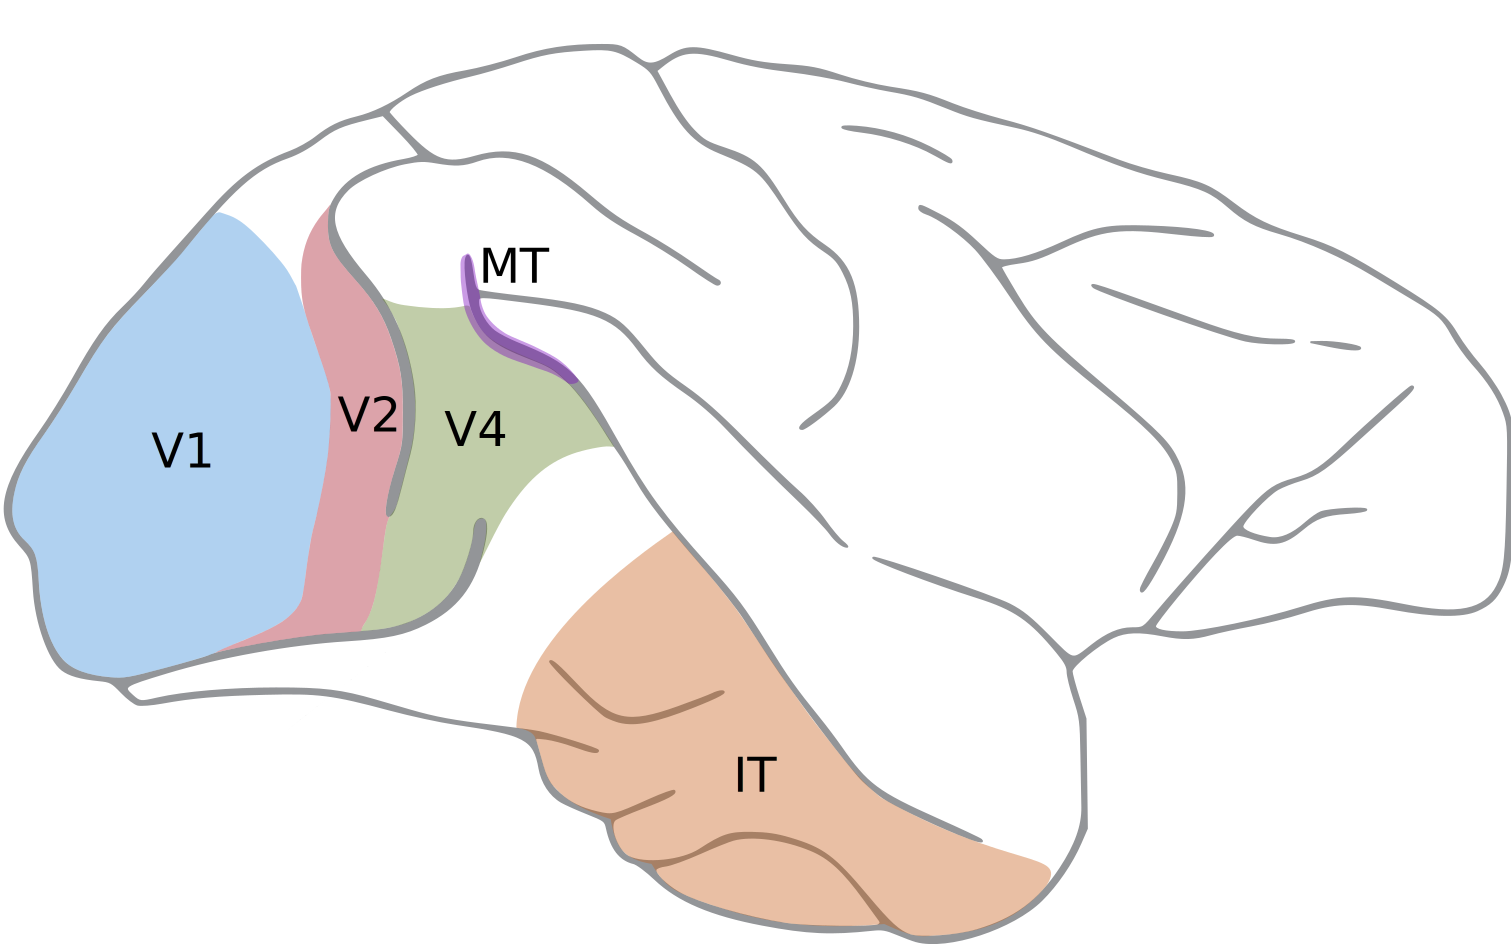
\includegraphics[width=86mm]{rhesusCerebrum.pdf}}
	\caption{\textit{The Rhesus Macaque Visual Hierarchy.} Each area depicted here is distinct in cytoarchitecture and maintains a complete retinotopic map. Information flows from the \gls{lgn} (not shown) to V1, then V2, V4, and finally the inferior temporal cortex (IT) in what we call the Ventral stream. }
	\label{fig:brain}
\end{figure}

It is known that each of these brain regions are unique and self-contained stages in hierarchical information processing. One reason they are thought to be unique stages is because each area has a full representation of the visual field (Retinotopic map) \citep{Felleman1997}. It has also been shown that neurons in these brain areas respond differently to the same visual information \citep{Mahon2001}, and have different functional architecture \citep{Yoshioka1996, Hubel1965}. At each stage of the hierarchy, the visual information is processed in increasingly complex ways. Information in photoreceptors is quite simple: it consists of how many photons of light there are at each point in the visual field. The \gls{rgcs} then sum that information and describe the first spatial derivative of the photoreceptors, where the changes in the concentration of light are (i.e. contrast edges; \cite{Wiesel1959}). The simplicity of this intra-areal computation is contrasted by the more intricate transformations between brain areas. For example, Hubel and Wiesel demonstrated that neurons in V1 respond dynamically to the orientation of a bar of light \citep{Hubel1959}, and so their firing rate contains information about orientation. Knowledge about the neural activity reduces the uncertainty about the stimulus and vice-versa. This stimulus-response relationship is the prototypical sensory coding function called a tuning curve. Studies have shown that the amount of stimulus information represented in the tuning curve of a neuron is highest at the peak (the stimulus that causes the highest firing rate) and the peak of the first derivative (largest slope), depending on the noise present in the system \cite{Butts2006}. Investigations into the neural code of the visual system therefore need to find stimulus dimensions that result in steep tuning curves and large peak responses from neurons. While bars of light are sufficient to investigate the neural code in early visual areas, these same stimuli are too impoverished to excite neurons in later areas. The low response rates are obstacles to describing the response function of neurons higher up in the visual hierarchy, like V4. The goal is still to find the domain in stimulus space that results in substantial, dynamic responses from a neuron, but the dimensionality of the stimulus space is astronomically larger. In the same manner that Hubel and Wiesel manipulated the width/orientation of a bar of light to excite V1 neurons, researchers have been developing novel strategies to make stimuli better suited for neurons in other visual areas \cite{Hubel1959, Pasupathy2002, Ponce2019, Cowley2017}. The resultant stimuli can be roughly categorized by the order of the underlying image statistics: first, second, and high-order. It is a precarious endeavor to match the complexity of a stimulus to the intricacy of a brain area's tuning preferences, but decades of work have guided a growing, cohesive understanding of stimulus-response functions. This work has lead to substantial improvements in sensory models of the brain as well as fundamental coding principles that generalize beyond the visual system.

%-----------------------------------
%	SUBSECTION 1
%-----------------------------------
\subsection{Subsection 1}



%----------------------------------------------------------------------------------------
%	SECTION 2
%----------------------------------------------------------------------------------------

\section{The Neural Response Function}
In its simplest form, one can consider visual neurons to be a biological implementation of some unknown function of a stimulus parameter ($\theta$):

\begin{equation}
R_n = f(\vec{\theta})
\end{equation}

%\begin{equation}
%f(\vec{\theta}) : \mathbb{R}^{n} \rightarrow \mathbb{R}
%\end{equation}

The neuron takes in inputs from dendrites, and produces an output in the form of action potentials (spikes). Computational neuroscientists then try to understand how the brain processes information by studying the input-output relationship of these functions. We begin with a single neuron, and a single variable input ($\theta$), to build the foundations for high-dimensional cases later.

\subsection{Tuning in One Dimension}

The prototypical representation of a neurons input-output function is the tuning curve. Tuning curves are estimated by taking discrete samples along a single feature dimension (orientation for example) and plotting the neural responses against the stimulus parameter (Figure \ref{fig:tuningIntro}A). In this case, each dot represents one trial of the stimulus-response function, and by averaging across trials we get an estimate (dotted line) of how a neuron responds to that stimulus dimension ($\theta$). This process provides the expected response of a neuron to each part of the stimulus space (Figure \ref{fig:tuningIntro}B) under the assumption that the tuning function is smooth where not sampled (\textbf{CITE FOR SMOOTH TUNING}). 
 
\begin{figure}[h]
	\centerline{\includegraphics[width=172mm]{tuningSamplingIntro.pdf}}
	\caption{\textit{Calculating a 1D Tuning Curve.} A.) The process for estimating a single neurons tuning curve to a single stimulus parameter $\theta$. Discrete stimulus values were chosen ($-180^\circ\ by\ 45^\circ\ to 180^\circ$) to span the stimulus space, and repeatedly presented (Gray dots). This provides the expected response to a given stimulus value (dotted line) for the neuron. B.) The estimated tuning and variability for the neuron in panel A.}
	\label{fig:tuningIntro}
\end{figure}

Importantly, this method also provides the reliability of the neural response function. While neurons are believed to respond in a deterministic manner, the presence of uncontrollable variables (biological noise \parencite{Faisal2008}, network oscillations \parencite{Fries2005}, latent factors \parencite{Yu2009, Chen2006}, etc.) makes most neurons appear to behave somewhat stochastically. That is, on any given trial, it may respond more or less than expected, which we call response variability. Tuning and variability both impact information signaling in unique ways, with different implications for the brain. 

A neurons tuning curve contains information. That is to say, knowledge of a neurons firing rate reduces uncertainty about the state of the world. Take the neuron from Figure \ref{fig:tuningIntro} for example. If the neuron is firing at $40\frac{spk}{s}$, it is pretty unlikely that the stimulus is either $0^\circ$ or $180^\circ$, so it is conveying information about the stimulus to other neurons. The question then becomes, \textit{how much} information a neuron is signaling. This quantity is directly related to three main components:

\begin{enumerate}
	\item Response Range
	\item Shape of tuning curve
	\item Response Variability
\end{enumerate}

The first point is addressed through natural upper and lower bounds. Neurons cannot have a negative firing rate, and neurons cannot fire arbitrarily fast due to biochemical constraints such as repolarization of chemical gradients and refractory periods (\cite{Kole2012}). The final two points are intertwined due to quantization of response and precision of readout. Neurons cannot fire half a spike, so a single neuron cannot encode to arbitrary precision (e.g. $45^\circ$ vs $45.000001^\circ$; remember that firing rates are bounded), even with 0 response variability. This makes properly utilizing the available range essential, i.e. the shape of the tuning curve.

\begin{figure}[h]
	\centerline{\includegraphics[width=172mm]{tuningAndInfo.pdf}}
	\caption{\textit{Tuning curves and Information.} A.) Von Mises tuning functions with different concentration parameters ($\kappa$). Color indicates highest information tuning functions for fine (Blue) and coarse (red) discrimination. B.) Mutual information (Firing Rate and orientation) as a function of $\kappa$. Blue line depicts $1^\circ$ discrimination, Red line depicts the more realistic situation of 8 stimulus classes ($0^\circ$ to $315^\circ$ in $45^\circ$ steps). }
	\label{fig:tuningInfo}
\end{figure}

Previous work has demonstrated that the most informative parts of a tuning curve is where the slope is highest \parencite{Series2004}. A small change in the stimulus results in the largest change in the response, making those sections the most sensitive to the stimulus dimension. Given this, one may fall into the trap of thinking larger slope means more information. Consider instead the black tuning curve in Figure \ref{fig:tuningInfo}A. If the task is to discriminate between $\theta=45^\circ$ and $\theta=90^\circ$, this is the worst stimulus-response function to use. In fact, the shape of a neurons tuning curve has been shown to vary with the demands on the system \parencite{Scott2023}. In the case of tuning width ($\kappa$ parameter of a Von-Mises function), course discrimination ($0^\circ$ vs. $45^\circ$) necessitates a wider tuning function than fine discrimination ($0^\circ vs. 1^\circ$; Figure \ref{fig:tuningInfo}B). This is because we are optimizing the tuning function for discrimination across the whole available range of $\theta$, not just the high-slope regions. 


%Neurons were modeled with an average response following \textbf{REFERENCE TO VON MISES EQUATION}. In this way, each stimulus value corresponds to an expected response (\textbf{LAMBDA}), which was then used as the rate parameter to pull trials from a poisson distribution.

\subsection{nD Stimulus Spaces: Multiple Features}
In the previous section I discussed the basics of tuning in 1 dimension. This explored how one neuron responds to changes in one stimulus parameter $\theta$. This is an oversimplification of the true process, as no true stimulus can be described with only a single number. In this section I will expand the concept of a 1D tuning curve to an nD tuning surface spanning multiple feature dimensions. 

\begin{figure}[ht]
	\centering{\includegraphics[width=172mm]{gabor2DStimSpace.pdf}}
	\caption{\textit{Gabors as points in a 2D Stimulus Space.} A.) examples of Gabor stimuli with various $\theta$ and spatial frequency values. B.) Positions of the Gabors depicted in panel A within a 2-Dimensional stimulus space. }
	\label{fig:gabor}
\end{figure}

One of the most heavily-studied and simplest stimuli used in studies of visual neuroscience is the Gabor (Figure \ref{fig:gabor}A). Gabors (or wavelets) are essentially oscillating light and dark patches at an orientation. These stimuli are often used in low-to-mid-level visual areas such as \gls{lgn} (\cite{Mahon2001}), V1 (\cite{Bredfeldt2002,Lennie1990, Tanigawa2010}), V2 (\cite{Gegenfurtner1996, Liu2020}) and \gls{mt} (\cite{Movshon1996, Rust2006}). Most such studies use the orientation dimension to produce tuning curves as described previously (Figure \ref{fig:tuningIntro}A), but many make necessary choices which limit them along non-studied feature dimensions (eg. spatial frequency, color, size, etc.). Let us begin with a 2D feature space by adding spatial frequency to orientation. Figure \ref{fig:gabor}A demonstrates how independently varying the two feature dimensions results in a set of stimuli that a particular neuron may be tuned for. These are of course discrete steps representing two continuous feature dimensions (orientation and spatial frequency). This results in an important conceptualization, the stimulus space (\ref{fig:gabor}B). Here, every possible combination of orientation and spatial frequency are represented as points in a plane. 

This is a natural progression from the 1-Dimensional orientation case shown before. All experiments investigating orientation tuning, necessarily limit stimuli along other dimensions. So while spatial frequency (for example) is kept constant in those experiments, neurons are likely still responding according to their n-dimensional tuning function. This results in a tuning surface (or tuning manifold in $>2$ dimensions), such as in figure \ref{fig:2Dtuning}. Here we have the same model neuron from \ref{fig:tuningIntro}, where it's tuning before was just a slice (gray plane) through some 2D surface.

\begin{figure}[h]
	\centering{\includegraphics[width=86mm]{2Dtuning.pdf}}
		\caption{\textit{Tuning along multiple Feature Dimensions.} A neurons tuning curve, in 2 dimensions becomes a tuning surface. Gray plane represents the spatial frequency value at which the tuning for $\theta$ matches figure \ref{fig:tuningIntro}.}
		\label{fig:2Dtuning}
\end{figure}

This idea of multidimensional tuning is more realistic, albeit more cumbersome. One of the biggest problems with studying neuron behavior this way is how intractable it is in 3+ dimensions. Take the 1D tuning curve in \ref{fig:tuningIntro}A. An experimenter must test the neural response function at several points to get an estimate of the tuning curve (in this case 8 orientations), because we do not know a priori which values along the stimulus dimension any one neuron is sensitive to. If, for example, we took the neuron from \ref{fig:tuningIntro}A and only sampled $\pm 90^\circ$, we would conclude that the neuron is not tuned to orientation. This is to say there is a minimum required sampling of each stimulus dimension we are interested in. Additionally, neurons often perform nonlinear operations \parencite{Carandini2012} so we must sample each relevant dimension independently. This means to get a meaningful tuning curve for an N-dimensional feature space requires around $8^n$ individual stimuli (assuming 8 sampled values for each dimension) sampled with repetition (5-10 trials each). So for a Gabor stimulus with feature parameters 1.) Orientation, 2.) Spatial Frequency, 3.) Color, 4.) Contrast, and 5.) Size, with the minimum 5 trials each, an experimenter would have to show $163,840$ stimuli in a single recording session. This is of course just for Gabors, one of the simplest visual stimuli. In more naturalistic settings, the number of feature dimensions could count in the hundreds. This problem motivates a more intelligent approach to searching for high dimensional feature tuning, which I will expand on in Chapter \ref{ch:optim}.


\subsection{nD Response Spaces: Multiple Neurons}

In the last section I built on the 1D neural response function by introducing the idea of multiple input dimensions: multiple features. In this section I will bring it back to 1 feature dimension, and discuss the implications of multiple response dimensions: multiple neurons.

Take again the example of neurons in V1 that are tuned for the orientation of a Gabor. This time we show a population of 8 neurons with equally-spaced preferences for $\theta$ (Figure \ref{fig:stateSpace}A). We can assume for the moment that each neuron independently contributes information about the value of $\theta$ with its' firing rate. A brain area or decoder with knowledge of all 8 neurons firing rates can accurately estimate $\theta$. For example, if neuron 1 has a low firing rate, and neuron 2 has a high firing rate, $\theta$ is most likely to be around $0^\circ$.

\begin{figure}[h]
	\centerline{\includegraphics[width=150mm]{stateSpace.pdf}}
	\caption{\textit{Population Codes} A.) Tuning curves for 8 homogenous model neurons along the orientation feature dimension. Color at the bottom represents the values of $\theta$. B.) A 2-Dimensional state space plotting the responses of neurons 1\&2 from panel A. Color represents the value of $\theta$ that lead to each pair of neural responses.  }
	\label{fig:stateSpace}
\end{figure}

This brings up another important concept that parallels the stimulus space from figure \ref{fig:gabor}B, the Neural state space \parencite{Paninski2010,Cross2021a}. A state space is a representation of neural data in which each dimension (or axis) is the firing rate of one neuron (Figure \ref{fig:stateSpace}B). We can then plot experimental variables (eg. stimulus features) according to the neural activity they elicited. In figure \ref{fig:stateSpace}B, $\theta$ is represented by color, and plotted according to the relative responses of neurons 1 and 2 from panel A. This plot also represents the simplest case of a 1-Dimensional response manifold \parencite{Kriegeskorte2021, Chung2018}. 

An important point to make here, as discussed in \textcite{Kriegeskorte2021}, is that tuning curves (Figure \ref{fig:stateSpace}A) determine the shape of the neural manifold (Figure \ref{fig:stateSpace}B), but not the other way around. Different sets of tuning curves are capable of generating the same manifold geometry. 


For example, if neuron 1\&2 from figure \ref{fig:stateSpace}A had the same tuning curve, adding neuron 2 provides no extra information. The fact that their preferences are offset is where the extra information comes from. This does not remain true when one considers response variability from before, as two identical neurons can provide multiple samples simultaneously (e.g. one neuron with two trials, or two identical neurons with one trial). 

Likewise, another major issue when expanding intuitions about tuning beyond a single neuron, are shared neural variability. When neurons co-vary together within stimulus condition, we call these noise correlations \parencite{Cohen2009, Ruff2016, Snyder2014, Moreno-Bote2014a}.


\subsection{Next Steps}
The bulk of this thesis resides in the final section of this introduction, comparing high dimensional neural and feature spaces. As discussed previously, many studies have looked into tuning of neural populations to single feature variables, and more still investigated individual neural tuning in multiple feature dimensions. Quite few have attempted to investigate both simultaneously, due again to intractability of the problem. 
In chapter \ref{ch:papernak}, I first discuss how even the simple case of neural tuning to one feature dimension is complicated by task demands and behavioral context. Then in chapter \ref{ch:optim} I expand on neural optimization techniques to elucidate tuning for multiple features from a population of neurons. I will also expand on how to interpret and analyzed such rich data using techniques such as \gls{cca} and \gls{dca} on simulated neural populations with known tuning parameters. Finally, in chapter \ref{ch:maps}, I apply all previous theory and techniques in a series of experiments aimed at deriving simultaneous understanding about both high-dimensional spaces. 






